%======================================================================
\chapter{MCL-WMR: a Comprehensive Motif-Recognition Algorithm}\label{chapter:mclwmr}
%======================================================================

In Chapter \ref{chapter:related_work} we described the motif-recognition problem in detail, and described several other motif-recognition programs.  Pevzner and Sze defined the weak motif-recognition problem more concretely by illustrating the limitations of most motif-recognition programs; their results illustrate that although most methods at the time were capable of finding motifs of length 6 with no degeneration, most failed to detect motif instances of length 15 with 4 degenerate positions in a random sample containing 20 sequences that were 600 nucleotides long \cite{PS00}.  Since these challenge problems were defined, many approaches were developed with the intention of detecting motifs that have a relatively large number of degenerate positions.  In this chapter we describe a new approach for this problem, and provide theoretical and experimental results that support our approach.

Our algorithm, MCL-WMR, builds a weighted graph model of the input data and uses a graph clustering algorithm to quickly determine important subgraphs that need to be searched further for valid motifs. We compare the results of MCL-WMR to that of previously developed approaches; testing on synthetic data has shown that MCL-WMR has competitive running time capabilities and accuracy.  An added advantage of MCL-WMR is the ability to detect multiple motif instances. 

As previous described, the {\sc Closest String} problem asks, given a parameter $d$ and a set $S = \{s_1, \ldots, s_n\}$ of $n$ strings, each of length $\ell$, whether there exists a string that has Hamming distance at most $d$ from each of the strings in $S$. The following definition will be useful in this and later chapters:

\begin{definition} {\bf (weight of a set of sequences)}\label{def:weight} Given a set $S = \{s_1, s_2, \ldots, s_n\}$ of $n$ sequences, each of length $\ell$, we define the {\em weight} of the set $S$ to be $\sum_{i = 1}^n \sum_{j = i}^n  \ell - d(s_i, s_j)$.  \end{definition}

For a given parameter $d$ we say $S$ is a {\em motif set} if there exists a center string $s^*$ at distance at most $d$ from any string in $S$; we say a set $S$ of strings is {\em pairwise bounded} if the distance between any pair of strings in $S$ is at most $2d$.  Every motif set is pairwise bounded; if a pairwise bounded set is not a motif set we say it is a {\em decoy set}.  For example, for $d=1$ the set $\{000, 001, 010, 100\}$ is a motif set because $000$ is a center string for this set.  In contrast, the set $\{000, 011, 101, 110 \}$ is a decoy set because it is pairwise bounded (since any two of the strings are at Hamming distance at most two) but no center string exists.  We introduce the exploration of using the weight of a set as an indicator of whether a {\sc Closest String} instance is a motif set or a decoy set. 

\section{System and Methods} \label{section:mcl_wmr_system}

MCL-WMR involves three stages: graph construction, clique finding using graph clustering, and recovering the motif instances and their center strings. An overview of MCL-WMR is shown as follows: 

\begin{algorithm*}
\caption{An overview of MCL-WMR}
\begin{algorithmic}
\STATE  \% build the graph from the given data
\STATE{\bf for }each of the subgraphs{ \bf do}
 \STATE \hspace{5mm}cluster subgraph using MCL
 	\STATE\hspace{5mm}{\bf for} each cluster {\bf do}
	\STATE\hspace{10mm}{\bf if} the weight of the current cluster is above $threshold$ {\bf then}
	\STATE\hspace{15mm}search that cluster to see if it contains a motif	
	\STATE\hspace{15mm}if we find a motif, we are done.
\end{algorithmic}
\end{algorithm*}

\noindent The MCL-WMR algorithm first chooses a {\em reference sequence} from the data set, denoted as $S_r$, building the entire graph from all the input data (including $S_r$), and for each vertex $v_{r \Sigma}$ representing the length-$\ell$ subsequence from $S_r$ starting at position $\Sigma$.  We then use the Markov Cluster Algorithm (MCL) \cite{vD00} to generate subgraphs which contain vertices that are highly inter-related. From these clusters of vertices we will generate the positions of the possible motif instances and their corresponding center string. The algorithm terminates when a motif is found.  In order to increase the probability that a motif is found, we minimize searching subgraphs with low probability of containing a motif; hence, the adjacency subgraphs are not clustered and searched in a sequential manner.
  
\subsection{Graph Construction}\label{graph_construction} 

In our graphical representation of the data set, each subsequence of length $\ell$ is represented by a vertex and the construction of our graph ensures that the motif instances represented by vertices in the graph are connected to each other and form a clique of size $n$ (though the converse need not hold).  Thus, the weak motif-recognition problem is converted to finding cliques with size $n$ in our constructed graph $G$ which is defined as follows:

\begin{enumerate}
\item The vertex set contains a vertex $v_{i,j}$ representing the $\ell$-length subsequence in sequence $i$ starting at position $j$, for each $i$ and $j = 1, 2, \dots, m-\ell+1$. There are $n(m-\ell+1)$ vertices.
\item Each pair of vertices $v_{i,j}$ and $v_{i',j'}$, for $i \neq i'$ is joined by an edge when the Hamming distance between the two represented subsequences is at most $2d$.
\item An edge between vertices having distance $k$ has weight $\ell - k$ for $d < k \leq 2d$, or $10(\ell-k)$ for $k \leq d$.  This emphasizes subsequences at small distances.
\end{enumerate}

\noindent This graph is represented by a symmetric adjacency matrix, where each entry is 0 for a non-edge, or a positive weight for an edge. This representation takes $O((n(m-\ell+1)^2))$ space and is constructed in $O(n^2(m-\ell)(m+\ell))$ time. Since the graph is $n$-partite, a clique of size $n$ contains exactly one vertex from each sequence. 

We reduce the size of the instance being passed to MCL by considering subgraphs $\{G_0, G_1, \dots, G_{m-1}\}$, where $G_i$ is the subgraph induced by the vertex corresponding to the reference sequence (denoted as $v_{R,i}$), and its neighbours (for some arbitrary choice of reference sequence $R$) instead of searching all of $G$ at once. Therefore, we have reduced the problem of finding weak motifs in the input data set $S$ to finding cliques of size $n$ in the $G_i$, though, some cliques may not correspond to valid motifs. Figure \ref{fig:graph_construction} illustrates this weighted graph construction of the input sequences.  

\begin{figure}[!h]
\begin{center}
 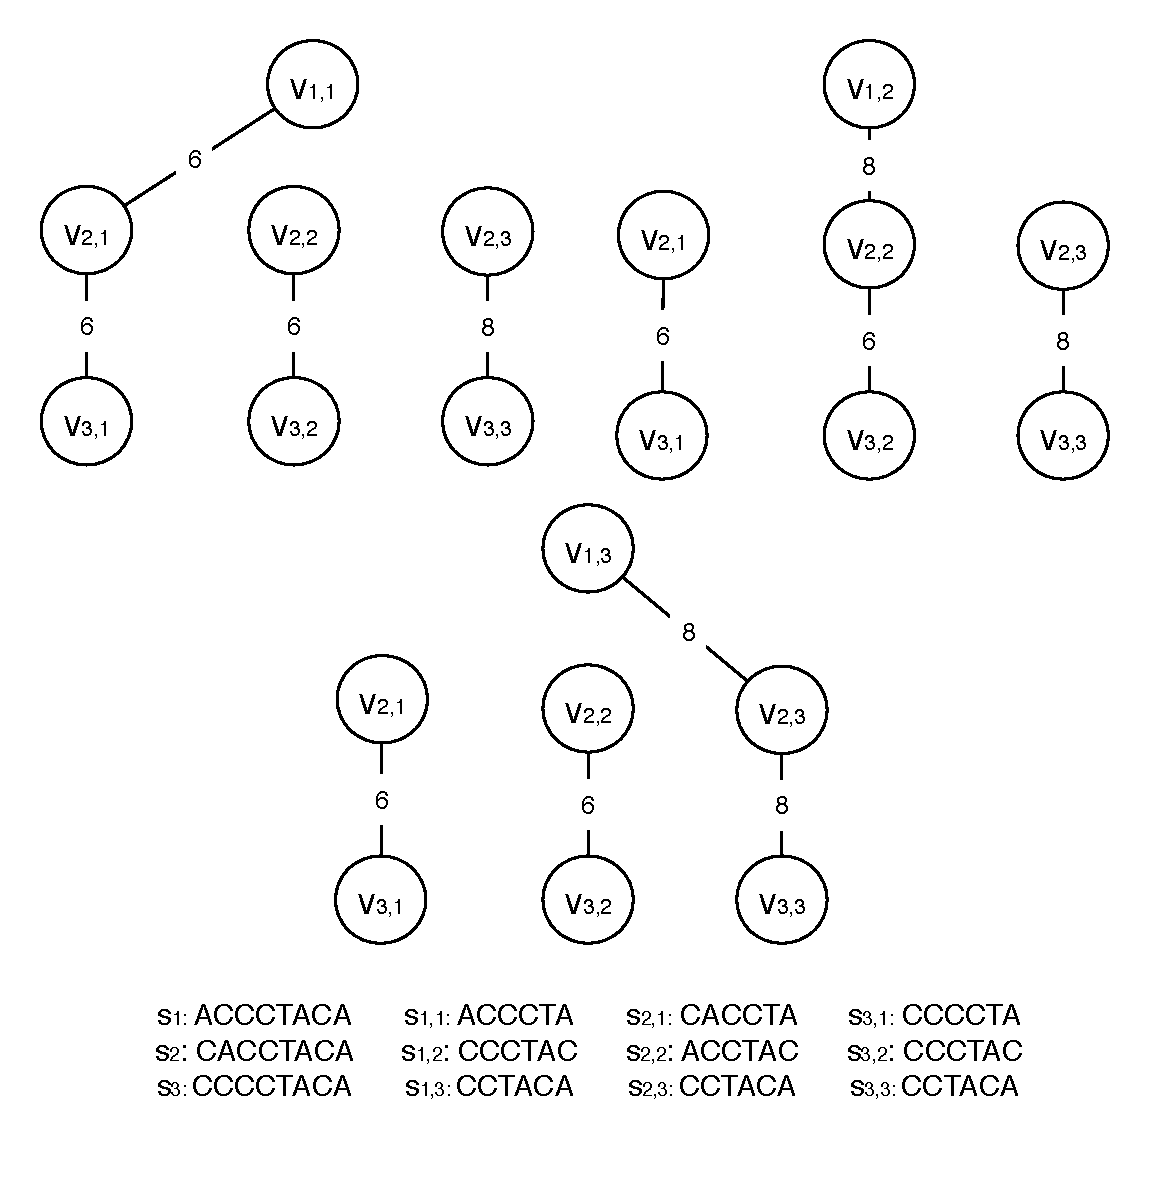
\includegraphics[width=\linewidth]{images/graph_construction}
\caption[An example showing the weighted graph representation of the input data used by MCL-WMR.]{An example showing the weighted graph representation of the input data used by MCL-WMR. The three input sequences are shown at the bottom-left corner of the figure. We have $n=3$, $m=8$, $\ell=6$, $d=1$. }
\label{fig:graph_construction}
\end{center}
\end{figure}

\subsection{Using Clustering to Find Motifs}

A {\em clustering} of graph is a decomposition of the vertex set into subsets of vertices that are highly intra-connected and, hence, induce dense subgraphs. A {\em good clustering} of a graph  is an approximation of a partitioning of the graph into cliques. A clique corresponding to a motif will exist in one of the subgraphs of $G$ since each motif instance appears as a vertex in a clique of size $n$.  We use MCL \cite{vD00} to cluster the sets of vertices to determine subgraphs that are highly intra-connected with high-weight edges, and sparsely inter-connected and thus likely to correspond to a motif instance.  We chose MCL because it is able to handle weighted graphs, and because it efficiently handles large undirected graphs. The idea underlying the MCL algorithm is that dense subgraphs correspond to regions where the number of length $k$ paths is relatively large, for small $k$. Random walks of length $k$ have higher probability for paths beginning and ending in the same dense region than for other paths.   

The MCL process consists of the alternation of two operations, namely {\em expansion} and {\em inflation}.  The image of a stochastic matrix under expansion is just some finite power of the matrix.  The image of a (column) stochastic matrix under inflation is formed by raising each entry of the matrix to the same positive power, followed by a rescaling of the columns such that the result is stochastic again.  An MCL process is defined by a column stochastic input matrix $T_1$ and two rows of exponents $e_{(i)}$, $r_{(i)}$, resulting in a row of stochastic matrices $M_{(i)}$, defined by:$$T_{2i} = \exp_{e_i} (T_{2i - 1}),  \,\,	i = 1, \ldots, n$$ $$T_{2i + 1} = \Sigma_{r_i} (T_{2i}),	\, i = 1, \ldots, n$$ where $\exp_{e_i}(T)$ is $T^{e_i}$ and $e_i \in \mathcal{N}$ and $r_i \in \Re$, $r >0$.  The image under the {\em inflation operator} $\Sigma_r$ of a nonnegative matrix $M \in \Re^{k \times \ell}$ having no zero columns is defined as: \[(\Sigma_rM)_{pq} = (M_{pq})^r \/ \sum^{k}_{i = 1} (M_{iq})^r. \] The largest transition probabilities will generally correspond with nodes lying in the same natural cluster; this effect is boosted in the MCL process via the inflation operator. By expansion, transition probabilities corresponding with random walks of higher length are computed.  The inflation operator promotes larger transition probabilities at the cost of small probabilities and thus, promotes random walks between nodes lying in the same cluster and demotes random walks between nodes lying in different clusters. 

\subsection{Recovering Motifs}

MCL produces sets of vertices that produce dense regions of the subgraph $G_i$; we filter the subgraphs obtained from MCL to subgraphs that have high probability of containing a motif.  A clique in $G$ that represents a motif instance must have size $n$ and have weight greater than or equal to $( \ell - 2d) {n \choose 2}$ since each pair of vertices are adjacent.  We filter out clusters that do not meet these criteria. Clusters that pass this test may contain multiple cliques formed by choosing different subsets of $n$ cluster vertices, or possibly no cliques at all. We identify all ways of forming a clique from the cluster vertices by using the $n$-partite nature of the graph to explore all possible cliques with the following depth-first search algorithm.  The dynamic-programming algorithm we use is as follows:

\begin{enumerate}
\item Let the sets $\mathcal{C} = {\mathcal{C}_r , \mathcal{C}_2, \ldots, \mathcal{C}_n}$ represent the subsets of vertices in a cluster that need to be considered.  Hence,  $\mathcal{C}_r = \{v_{r\sigma}\}$, $\mathcal{C}_2 = \{v_{21'} , v_{22'}, \ldots, v_{2|\mathcal{C}_2|'} \}$, $\ldots$, $\mathcal{C}_n = \{v_{n1'} , v_{n2'}, \ldots, v_{n|\mathcal{C}_n|'} \}$. Note that $\mathcal{C}_r$ contains only one vertex since it is the reference sequence. 
\item Lists $\mathcal{L}_{ij'}$, for $i = r$ and $j' = \sigma$ and $i = 2, \ldots, n$ and $j' = 1, \ldots, |\mathcal{C}_i|$ are created as follows: 
\begin{enumerate}
\item Set $\mathcal{L}_{r\sigma} = \emptyset$. 
\item Set $\mathcal{L}_{2j'} = \{v_{r\sigma} \}$ for vertex $v_{2j'} \in \mathcal{C}_2$. 
\item for $i = 3, \ldots, n$ 
\begin{description}
\item[~] Set $L_{ij'} = \emptyset$ for $v_{ij'} \in \mathcal{S}_i$
\item[~] for each vertex $v_{i -1k'} \in \mathcal{C}_{i−1}$, $k' = 1, \ldots, |\mathcal{C}_{i−1}|$
\begin{itemize}
\item if $d(v_{ij'}, v_{i-1k'} ) \leq 2d$ then let $\mathcal{L}_{ij'}$ be equal to $\mathcal{L}_{ij'} \cup \{ v_{i-1k′} \} \cup \mathcal{L}_{i-1k'}$
\end{itemize} 
\end{description}
\end{enumerate}
\item If a clique with size $n$ exists then there must exist a list $\mathcal{L}_{nj'}$ for vertices $v_{nj'} \in \mathcal{C}_n$ that contains vertices from each set $\mathcal{C}_i$ for $i = 1, \ldots, n -1$. 
\end{enumerate}

For each such clique found using the above dynamic-programming algorithm, we test if it represents a motif instance by attempting to find a string that has distance at most $d$ to every vertex. We do this by building up a list of possible center strings and the number of mismatches to each vertex for each possibility, one character at a time. Once a candidate string has $d+1$ mismatches to some vertex, it is discarded. Although the space of $4^{\ell}$ possible center strings is very large, in practice the list is pruned very rapidly on the $d+1$st character, {\em i.e.}\ after reaching size $4^d$.

We use a heuristic to determine a center string which tries all possible length $\ell$ DNA sequences that have high probability of having distance at most $d$ from each string in the set $S$ and thus, determines whether the subsequences are $(\ell, d)$-motifs.  In practice this dynamic-programming algorithm is quite efficient because the size of the clusters returned by MCL is small.  After obtaining the possible motif instances from $s_n$, the corresponding likely center string is found by alignment of the $n$ sequences and lastly, in order to determine if the set of subsequences found are motif instances it is checked that each subsequence is of distance at most $d$ from the center string.  As the sequences become longer or $d$ becomes large relative to $\ell$, the number of spurious cliques found will increase; this final step guarantees that the found subsequences are proper motif instances. 

\section{Analysis of Graph-Theoretic Model}

To validate our approach of using edge weights to assist in the search of valid motifs we show the existence of a separation between the weight of a set of sequences corresponding to a motif set and that of a set of sequences that does not correspond to a motif set.  We prove that the weight of an arbitrary set of subsequences corresponding to a motif set deviates from the mean with low probability.  Empirical results support the analytical description of the distribution and show that for a  typical motif-recognition problem ({\em i.e.} when $\ell = 15$ and $d = 4$) there exists a separation between the distribution of the weights of the motif sets and those of the decoy sets.

\subsection{Analysis of the Weight of a Clique Containing a Motif} \label{section:mcl_wmr_analysis}
 

Consider a clique $C$ that contains a set of subsequences corresponding to a motif set. Let $W$ be the random variable for the sum of each of the ${n \choose 2}$ edge weights in $C$. Let $v_1, v_2, \ldots v_n$ be the set of $n$ vertices in $C$ corresponding to sequences $s_1, \ldots, s_n$.  We seek the mean of $W$ and a tail bound for large deviations from the mean.  Let $W_i$ be the expected value of the random variable $W$ given that the first $i$ subsequences in $C$ are known.  

We prove several results concerning random $(\ell, d)$-motif sets.  A standard method used to generate a random $(\ell, d)$-motif set is to choose an $\ell$-length sequence uniformly at random from all possible $|\Sigma|^{\ell}$ sequences to be the center string, and then form a motif set by selecting $n$ sequences at random with replacement from the set of all sequences with Hamming distance at most $d$ from this center string \cite{BT02}.  This samples motif sets with probability proportional to the number of distinct center strings it has and thus, corresponds to how synthetic problem data sets are constructed and how we expect meaningful motif sets arise in nature.  For example, synthetic problem instances are traditionally generated as follows: a random center string of length $\ell$ is chosen, $n$ occurrences of the motif are generated by randomly mutating at most $d$ positions, and each of the $n$ motif instances is embedded at a random location into a different background string of length $m$.  We note that other non-uniform distributions have also been used to generate motif sets \cite{PS00}. 

\begin{theorem}  \label{mean_thm} The expected weight of a clique in $G$, which models a random $(l,d)$-motif problem containing $n$ sequences, is  \[ E[W] = {n \choose 2} \left( \ell -  \frac{1}{\beta^2}  \sum_{a=0}^{d} \sum_{b=0}^{d}{{\ell} \choose b}{{\ell} \choose a}3^{a + b} \left(  a+b-\frac{4ba}{3l}\right) \right) \] where $\beta= \sum_{i = 0}^{d} {{\ell} \choose i} 3^i$. \end{theorem}

\begin{proof} Given an $(\ell, d)$ motif set $S$, we aim to compute the expected value of the weight of the set $S$ ({\em i.e.} $E[\sum_{i=1}^{n}\sum_{j=i+1}^{n}(\ell - d(s_i,s_j))]$.  Let $\mu_e$ be $E[d(s_i,s_j)]$ for any pair of sequences $s_i$ and $s_j$, where the corresponding vertices $v_i$ $v_j$ are joined by an edge in the clique that contains $S$.

\[ E \left[ W \right] =  E \left[ \sum_{\forall v_i, v_j, i < j} (\ell - d(s_i, s_j)) \right] = {n \choose 2} \mu_e \]
 
We choose the $n$ sequences uniformly from the $\beta = \sum_{i = 0}^{d} {{\ell} \choose i} 3^i$ possible choices. Let $s$ be a center string for the $\alpha_i$ denote the Hamming distance between $s_i$ and the center string $s$.  The expected weight of an edge will depend on the distance of the two sequences from the center string, so we break the expectation into pieces, as follows:

\begin{center}
\begin{math}	
\begin{array}{lll}
\mu_e  	& = & \sum_{\alpha_i = 0}^{d}\Pr[d(s, s_i) = \alpha_i ] E[d(s_i,s_j)| d(s, s_i) =\alpha_i ] \\
					& = & \sum_{\alpha_i = 0}^{d}\Pr[d(s, s_i) = \alpha_i ] \cdot  \sum_{\alpha_j=0}^{d}\Pr[d(s, s_j) = \alpha_j ]  \\
                    & ~  &  E[d(s_i,s_j)|d (s, s_i ) = \alpha_i, d (s, s_j ) = \alpha_j ] \\
					& = & \sum_{\alpha_i = 0}^{d}\frac{ {{\ell} \choose {\alpha_i}}3^{\alpha_i}}{\beta}\sum_{\alpha_j=0}^{d}\frac{{{\ell} \choose {\alpha_j}}3^{\alpha_j}}{\beta}E[d(s_i,s_j)|d (s, s_i ) = \alpha_i, d(s, s_j ) = \alpha_j ] \\
\end{array}
\end{math}
\end{center}	

The remaining problem is to compute the expected Hamming distance between $s_i$ and $s_j$, knowing that the sequences consist of copies of $S$ with $a$ and $b$ positions mutated, respectively. If a position was mutated in neither string it is a match; if a position was mutated in one sequence but not the other it is a mismatch; if a position was mutated in both sequences, it is a match with probability $\frac{1}{3}$.

If $s_i$ is fixed, $s_j$ consists of $b$ mutations that each either hit one of the $a$ mutated positions in $s_i$ or one of the other $\ell - a$ positions, sampled without replacement. The number that hit the $a$ mutated positions in $s_i$ follows a hypergeometric distribution with mean $\frac{ba}{\ell}$. If the number of hits to mutated positions is $c$, the expected total number of mismatches is: $b-c$ positions that hit among the $\ell-a$ non-mutated positions in $s_i$, $a-c$ positions among the $a$ mutated positions of $s_i$ that were \emph{not} hit, and $\frac{2}{3}c$ mismatches from the hits among the mutated positions, for a total of $(b-c)+(a-c)+\frac{2}{3}c = a+b-\frac{4}{3}c$. Therefore, $E(d(s_i,s_j)|d(s,s_i)=a, d(s,s_j)=b) = a+b-\frac{4ba}{3\ell}$. 

Therefore, $\mu_{e}$ is equal to $\ell -  \frac{1}{\beta^2}  \sum_{a=0}^{d}{{\ell} \choose a}3^a\sum_{b=0}^{d}{{\ell} \choose b}3^b \left(  a+b-\frac{4ba}{3\ell} \right) $, the expected weight of a single edge. 

\begin{center}
\begin{math}	
\begin{array}{lll}
E \left[ W \right] 	&=& {n \choose 2} \left( \ell -  \frac{1}{\beta^2}  \sum_{\alpha_i=0}^{d}{{\ell} \choose {\alpha_i}}3^{\alpha_i}\sum_{\alpha_j =0}^{d}{{\ell} \choose \alpha_j}3^{\alpha_j} \left(  \alpha_i+ \alpha_j-\frac{4\alpha_i \alpha_j }{3\ell} \right) \right) \\		
 							&=& {n \choose 2} \left(\ell -  \frac{1}{\beta^2}  \sum_{\alpha_i =0}^{d} \sum_{\alpha_j =0}^{d}{{\ell} \choose {\alpha_j}}{{\ell} \choose {\alpha_i}}3^{\alpha_i + \alpha_j} \left(  \alpha_i +\alpha_j - \frac{4\alpha_i \alpha_j }{3l}\right) \right) \\		

\end{array}
\end{math}
\end{center} \hfill $\Box$	\end{proof}

We are able to bound the probability of $W$ deviating from its mean by first demonstrating that $W_0, W_1, \ldots,$ $W_n$ is a martingale sequence and next, applying Azuma's inequality \cite{MR95} to determine the probability of a specific deviation.

\begin{theorem}  \label{azuma_thm} Consider the $(\ell,d)$-motif problem containing $n$ sequences. Let $W$ be the sum of the ${n \choose 2}$ edge weights in an arbitrary clique in $G_{motif}$ that corresponds to a motif set and let $\mu_W$ be the expected weight of the motif set, then for any $\lambda > 0$,  
\[\Pr[|W - \mu_W| \geq \lambda] \leq 2 \exp \left( - \frac{\lambda^2}{2d^2(n + 1)}  \right) \]
\end{theorem}

\begin{proof} Recall that $W_i$ is the expected value of the random variable $W$ given that the first $i$ sequences in $C$ are known and hence, the distances between the center string $s$ and the first $i$ vertices are known. Without loss of generality we choose a center string $s$ and let $\mathrm{F}_i$ be the $\sigma$-field generated by the random choice of the sequence $s_i$ from the set of all sequences at most distance $d$ from $s$.  It follows that, $W_i = [W | \mathrm{F}_i]$ since $W_i$ denotes the conditional expectation of $W$ knowing the first $i$ subsequences and therefore, $W_0, W_1, \ldots, W_n$ is a martingale sequence \cite{MR95}, with $W_0 = E[W]$ and $W_n = W$.

We now focus on the value $W_i - W_{i - 1}$.  Let $\Delta_{i, e}$ be the change in the random variable representing the weight of an edge $e$ from knowing the first $i -1$ sequences to knowing the first $i$ sequences. The value of $\Delta_{e, i}$ is non-zero for edges where the sequence corresponding to one of the endpoints of that edge was previously not known and is now known.  Each vertex in the clique is adjacent to $n - 1$ vertices; $i - 1$ of these vertices have corresponding sequences that were known and $n - i$ of these vertices have corresponding sequences that were unknown; all other ${n \choose 2} - n + 1$ remaining edges in the clique have no change in the expected value. In both cases, the expectation of the weight of the edge can change by at most $d$. Again, $\mu_{e}$ is the expected value when neither sequences $s_i$ or $s_j$ corresponding to the endpoints of the edge $e = (s_i, s_j)$ are known and therefore, we have the following: 

\[ |W_{i} - W_{i - 1}| \leq \Delta_{i, e} (n - 1)  = d (n - 1) \]
 

\noindent We have shown that the random variables $W_0, W_1, \ldots, W_n$ form a martingale with $W_0 = E[W]$ and $W_n = W$ and that $|W_i - W_{i - 1}| \leq d(n - 1)$ and therefore, we can invoke Azuma's inequality \cite{MR95} to give us the following for any $\lambda  > 0$:

\[ \Pr\left[ |W - \mu_W| \geq \lambda \right]  \leq  2 \exp \left( - \frac{\lambda^2}{2 \sum_{i = 0}^n d^2} =  \right) =  2 \exp \left( - \frac{\lambda^2}{2d^2(n + 1)}  \right). \] \hfill $\Box$ \end{proof}

%\begin{figure}[h]
%\begin{center}
 %\includegraphics[width=170mm]{images/fig1}
%\caption[Distribution of the weight of cliques]{Distribution of the weight of cliques containing a center string and the distribution of the weight of cliques not containing a center string.  The data for non-motif cliques was generated was generated by running MCL-WMR 100 times, calculating the total weight of the clique, and generating a histogram of these values. The data  is given for the (15,4) motif problem instance with $n = 15$.  }
%\label{fig1}
%\end{center}
%\end{figure}
 
We can compare this theoretical tail bound with the distribution of the values obtained from MCL-WMR. Figure \ref{chapter4:fig2} demonstrates that as the value of $n$ increases, the deviation of the weight of cliques corresponding to motifs will occur with less probability, and the weight of the cliques will become more centralized around the mean.  Similar experimental tests were completed to demonstrate the relationship between the weight of spurious cliques when $n = 15$ and when $n = 50$, specifically, we ran MCL-WMR 100 times with $m = 800$, $\ell = 15$, and $d = 4$ and determined cliques that did not correspond to valid motifs. We found no spurious cliques in the data sets when $n = 50$, agreeing with our intuition that very few spurious cliques occur randomly in the data set when $n$ becomes large. 

We note our confidence in MCL-WMR being able to detect cliques -- both spurious and those corresponding to motifs -- this is due to the accuracy in detecting the embedded motifs (see Section \ref{results} details concerning these experimental tests).  These results also suggest that when $n$ is relatively large we can be more certain that any cliques found correspond to valid motifs (an attribute that will be further explored in this thesis).  

\begin{figure}[h*]
\begin{center}
 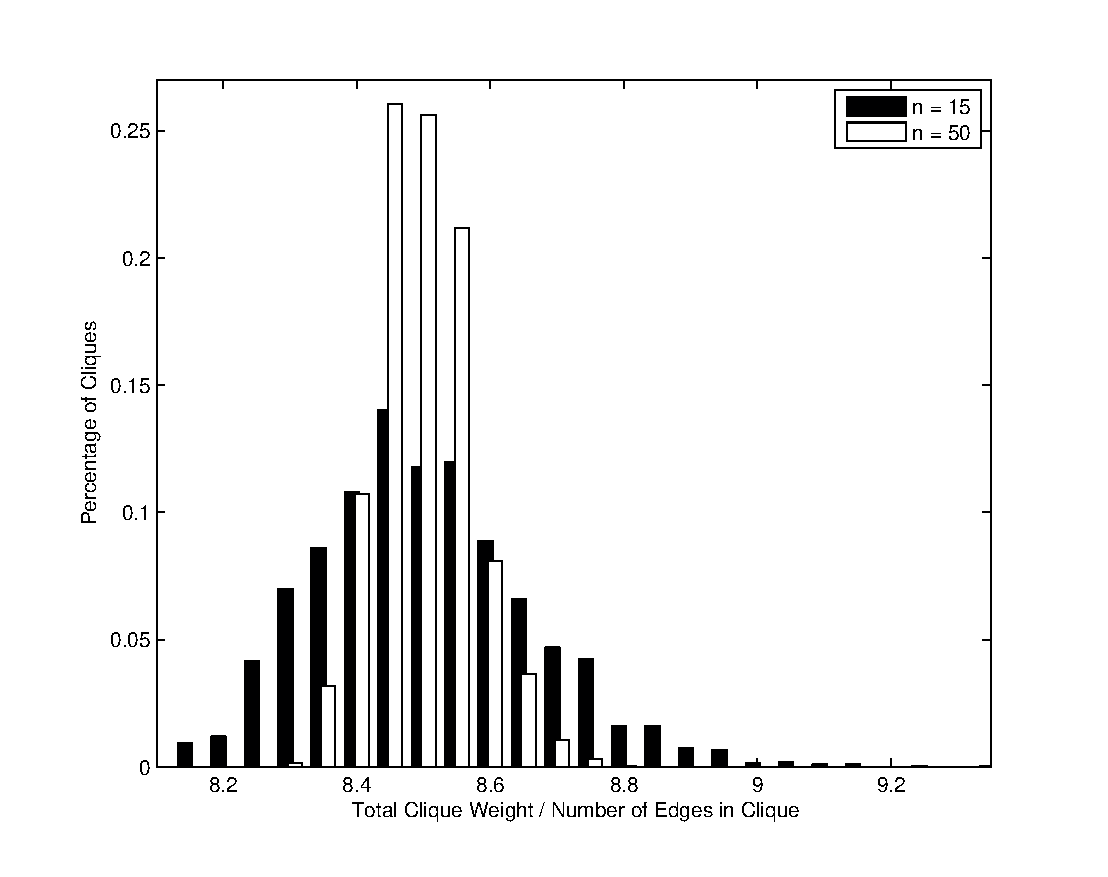
\includegraphics[width=\linewidth]{images/ex_n50a}
\caption[Data illustrating the distribution of the mean weight of an edge in a clique that corresponds to a valid motif set of size 15 and 50.]{Data illustrating the distribution of the mean weight of an edge in a clique that corresponds to a valid motif set  of size 15 (shown in black) and 50 (shown in white). The data is given for the $(15,4)$-motif problem with $m = 600$.  }
\label{chapter4:fig2}
\end{center}
\end{figure}

% Figure \ref{fig1} demonstrates that the distribution of the values of $W$ approach the normal distribution in the limit with the mean value entered at 897. This corresponds to the theoretical mean of 900.1 calculated using the result from Theorem \ref{mean_thm}.  Similarly, the weight of cliques that do not represent valid motifs follow a normal distribution, but the mean weight is approximately 885. This result, shown in Figure \ref{fig1}, was determined by generating the weight of the cliques that do not correspond to motifs in 100 random data sets , using MCL-WMR they are likely are not an uniform sample of all such cliques. 

\subsection{Discussion of Complexity}

A few interesting observations can be made regarding the complexity of the algorithm and the quality of its solutions. Finding cliques of maximum size in a given input graph is NP-complete and thus, unlikely to be solved in polynomial-time \cite{GJ}. Further, the results from Chen {\em et al.}\ \cite{CHKX04} show that unless unlikely consequences occur in parameterized complexity theory, the problem of finding maximum -- size cliques cannot be solved in $n^{o(k)}$ time. Thus, of finding cliques of size $k$ is not likely to be computationally feasible for graphs of significant size.  The best known algorithm for finding cliques of size $k$ in a given input graph runs in time $O(n^{ck/3})$, where $c$ is the exponent on the time bound for multiplying two integer $n \times n$ matrices; the best known value for is $c$ is 2.38 \cite{N02}.  

The running time for the straightforward algorithm that checks all size $k$ subsets is $O(n^{k+2})$ and is the one to be most likely to be implemented in practice.   The running time of the algorithm of  Yang and Rajapakse \cite{YR04}, a dynamic programming clique finding algorithm, is $O(n(mA^2 + A^{m - 1} p^{2m - 5})$, where $A = n \sum^{2d}_{i = 0}{{\ell}\choose i}(3/4)^i(1/4)^{\ell - i}$, $n$ is the length of each sequence and $m$ is the number of sequences.  This running time reflects the steep computational expense required to find cliques of a given size for an input graph.  Similarly, the estimated running time of the WINNOWER algorithm is $O((n D)^4)$, where $D$ is approximately $30$ for the challenge problem \cite{PS00}.  
 
The time required by MCL-WMR to find a solution is not affected directly by the length of the motif that is to be discovered, as is true of many other methods.  Rather, it is the weakness of the motif -- that is, the probability of the pairwise motif similarity occurring randomly -- that has the most impact on the complexity of the algorithm; the increased probability of a clique of high weight affects the running time of MCL-WMR since the exponential-time algorithm required to determine in a high cluster or subgraph contains a motif instance. 

We can compare the computational complexity of these programs by considering the required running time of MCL-WMR of the three sequential steps--that is, the computational time required to construct the graph, finds all cliques of size $n$, and determine the motifs and center string.  Other graphical methods of motif finding rely on an enumeration method to find dense subgraphs, including WINNOWER that requires each edge to be checked, and the algorithm of Yang and Rajapakse that uses dynamic programming on the complete graph. MCL-WMR omits this computational intensive work by employing MCL, which runs in time $O(N^3)$, where $N$ is the number of vertices of the input graph \cite{vD00}.  Hence, the most computationally expensive step is the clique-finding function, whose computation time increases with the number of vertices.

\section{Experimental Results}

We tested MCL-WMR on synthetic problem instances generated according to the embedded $(\ell, d)$-motif model. We produce problem instances as follows: first we choose a random string of length $\ell$, and pick $m$ occurrences of the motif by randomly choosing $d$ positions per occurrence and randomly mutating the base at each.  Lastly, we construct $m$ background sequences of length $n$ and insert the generated motifs into a random position in the sequence.  For each of the $(\ell,d)$ combinations, 100 randomly generated sets of input sequences ($n = 20$, $m = 600$) were generated.  An entry ``-'' indicates that the program was unable to solve the specific problem in a reasonable amount of time.
 
Our program found the exact location of a motif instance every single time and therefore, the performance coefficient is 1.  Other programs we tested did not achieve a performance coefficient of 1 and thus, returned approximate solutions to the embedded motif. The computation time of previous programs that find the exact solution becomes unacceptable as the motifs become degraded beyond the $(15,4)$ problem \cite{SJ04}.  For example, in 2004 Styczyski {\em et al.}\ \cite{SJ04} solved the $(17,5)$ problem exactly but took  greater than 3 weeks to do so and similarly, solving the $(14,4)$ took longer than 3 months (when $n = 20$ and $m = 600$).  The main advantage to our tool is the ability to solve the extremely difficult challenge problems (see Table \ref{performance1}).  See Subsection \ref{challenge_problems_section} for description of the term ``challenge problem''.


\begin{table}[h]
\begin{center}
\begin{tabular}{|c|c|c|c|c|c|c|}
\hline
$(\ell, d)$ & Gibbs & PROJECTION & SP-STAR & WINNOWER & MCL-WMR  \\
\hline 
(10, 2) & 0.150 & 0.80 & 0.56 & 0.78 & 1.00\\
(11, 2) & 0.68 & 0.94 & 0.84 & 0.90 & 1.00 \\
(12, 3) & 0.03 & 0.77 & 0.33 & 0.78 & 1.00 \\
(13, 3) & 0.60 & 0.94 & 0.92 & 0.92 & 1.00 \\
(14, 4) & 0.02 & 0.71 & 0.02 & 0.02 & 1.00  \\
(15, 4) & 0.19 & 0.93 & 0.73 & 0.92 & 1.00  \\
(17, 5) & 0.158 & 0.93 & 0.69 & 0.03 & 1.00 \\
(18, 6) & - & - & - & - &  1.00  \\
\hline
\end{tabular} 
\end{center}
\caption[Comparison of accuracy of MCL-WMR to other well-known motif-recognition programs on several challenge problems.]{Comparison of the performance on a range of $(\ell,d)$-motif problems with synthetic data.  Data from other algorithms are from Buhler and Tompa \cite{BT02}.  MCL-WMR, GibbsDNA, WINNOWER, and SP-STAR are averaged over eight random instances, while PROJECTION is averaged over 100 random instances.  In all these examples, $n = 20$ and $m = 600$.  }
\label{performance1}
\end{table} 


\begin{table}[h!]{
\begin{center}
\begin{tabular}{|c|c|c|}
\hline
$m$ & PROJECTION &  MCL-WMR\\
\hline 
600 & 2410 / 102  			& 2208 / 34 \\
800 & 2662 / 121			& 2802 / 42 \\
1000 & 2819 / 131			& 3223 / 89 \\
1200 & 3404 / 139 			& 3823 / 102\\
1400 & 3808 / 154 			& 4038 / 150 \\
1600 & 4310 / 159 			& 5037 / 167 \\
1800 & 4861 /  167 		& 4502 / 182 \\
2000 & 5012 / 182 			& 5001 / 201 \\
\hline
\end{tabular} 
\end{center}}
\caption[Comparison of the time required by MCL-WMR and PROJECTION to solve the $(15, 4)$-motif problem with 20 sequences of varying length.]{Comparison of the time required by MCL-WMR and PROJECTION to solve the $(15,4)$-motif problem with 20 sequences and $m$ varying between 600 to 2000.  The mean and standard deviation of the running time in CPU seconds is given. The success rate for PROJECTION was between 0.80 and 0.88.}
\label{n_table}
\end{table} 

The performance coefficient, which are shown for the various programs tested in Tables \ref{performance1}, \ref{n_table}, and \ref{performance2}, describe the fraction of  correctly solved instances and is described previously Subsection \ref{approximate_solution_section}. The performance coefficient of MCL-WMR is greater than that of the previous algorithms in every line of Table \ref{performance1}.  MCL-WMR correctly solved planted $(11,2)$, $(13,3)$, $(15,4)$, $(17,5)$ and $(18,6)$ on all data sets -- in these cases, the planted motif and motif occurrences at least as strong as planted motifs. WINNOWER, PROJECTION, and SP-STAR achieve acceptable performance on the $(11,2)$, $(13,3)$ and $(15,4)$ problem instances when the sequence length is less than or equal to 600 and the number of sequences is less than or equal to 20. However, all fail on the $(18,6)$ and $(19,6)$ problem, and WINNOWER and SP-STAR fail on the $(16,5)$ and $(17,5)$ problem instances.  The performance of MCL-WMR is best on the more difficult planted $(14,4)$, $(16,5)$, $(17,5)$ and $(18,6)$ motif problems when compared to results from previous algorithms.  WINNOWER and SP-STAR typically failed to find the planted motifs and PROJECTION often failed to have acceptable performance on the more difficult cases of the challenge problem \cite{BT02} and hence, MCL-WMR's performance substantially exceeded that of previously algorithms. 

We evaluated the performance of MCL-WMR on problem instances with longer background sequences -- that is, problems where $m$ varies from values greater than 600. As the length of the sequences increase, the number of randomly occurring $\ell$-mers increases; specifically, the increase in $m$ increases the probability of cliques of high-weight occurring. MCL-WMR will recover more computation time since the graph size will increase with the size of $m$.  Our results demonstrate that the computation time is comparable to that of PROJECTION, however, MCL-WMR is significantly more accurate than PROJECTION.  See Table \ref{n_table} for an illustration of these results.  Considering the $(15,4)$ motif problem and fixing the number of sequences to be 8, CONSENSUS, GibsDNA, and MEME have an unacceptable performance rate ({\em i.e.}\ below 0.7) when the sequence length increases to 300 or 400, the performance of WINNOWER breaks at length 700, and SP-STAR breaks when the length is 800 to 900. 
 
\begin{table}[h!]
\begin{center}
\begin{tabular}{|c|c|c|}
\hline
$(\ell, d)$ 	& PROJECTION 					& MCL-WMR  \\
\hline 
(10, 2) 			& 400 / 38	(0.98)			& 687 / 32 \\
(11, 2) 			& 670 / 43	(0.98)			& 1023 / 34 \\
(12, 3) 			& 1020 / 83 (0.87)			& 1442 / 52 \\
(14, 4) 			& 1521 / 95 (0.88)			& 1623 / 78 \\
(17, 5) 			& 5242 / 132 (0.78)			& 3023 / 103 \\
(18, 6) 			& -									& 5132 / 120 \\
\hline
\end{tabular} 
\end{center}
\caption[Comparson of the time required by MCL-WMR to PROJECTION to various motif challenge problems.]{Comparson of the running time of MCL-WMR to PROJECTION on various motif challenge problems. In all these examples, $n = 20$ and $m = 600$.  The mean and standard deviation of the running time in CPU seconds is given.  The success rate for PROJECTION is included in brackets. }
\label{performance2}
\end{table} 
\label{results}

	
\section{Summary and Open Problems}

We proposed an efficient algorithm for motif-recognition, whose specific purpose is to solve instances where there exists a large amount of degeneration with respect to the motif length.  We demonstrated promising results on synthetic data.  Specifically, we showed promising running time and accuracy for all challenge problems, with most-impressive improvement on the $(14,4)$, $(17,5)$ and $(18,6)$ problems.  Previous algorithms lack accuracy and efficiency in solving all challenge problems.  

Most importantly, we gave a novel model and framework for solving motif recognition instances that we will consider and study further in this thesis.  By changing the graphical model to incorporate edge weights, we can exploit theoretical results demonstrating the existence of a separation between the weights of cliques corresponding to valid motifs and the weights of those that do not, and obtain improved search techniques.   Our theoretical work and empirical data show a large percentage of the cliques corresponding to valid motifs have total weight in a narrow range.  This helps us distinguish cliques containing valid motifs and spurious cliques.  

The largest area for further improvement of MCL-WMR is the recovery of the motifs.  The dynamic-programming algorithm that explores the dense subgraphs to determine which subgraphs correspond to motif sets, and which correspond to decoy sets requires exponential time.  Note that this deciphering of subgraphs essentially reduces to solving instances of the {\sc Closest String} problem.  Next, we aim to create, analyze, and employ efficient algorithms for the {\sc Closest String} problem.  
